%!TEX root = thesis.tex


\chapter{Agent Stability}
\label{chapter3}

As was previously mentioned, requiring long training time and having poor initial performance have prevented RL from being widely adopted beyond research settings. Additionally, lack of stability guarantees prevents application of trained agents to safety critical applications. This chapter presents a numerical stability analysis of the learned controllers and shows how the combined controller architectures affect stability.
%
There are a variety of notions of stability that have been developed. Bounded-Input-Bounded-Output (BIBO) and Lyapunov stability were used to evaluate the performance of the controllers that were introduced in Chapter~\ref{chapter2}.

\section{Stable in the Sense of Lyapunov}

% Stability can be generally described as the tendency of a system to stay near an equilibrium.
% We can start the analysis of the stability of the combined controllers using Lyapunov stability.
In order for a system to be stable in the sense of Lyapunov, a system that begins in the neighborhood of an equilibrium, $x_e$, must remain near the equilibrium. This notion of stability is defined formally as:
%
\begin{equation}
  ||x(t_0)-x_e||<\delta \quad \text{and} \quad ||x(t)-x_e||<\epsilon \quad \forall t>t_0
\end{equation}
%
where $\delta$ and $\epsilon$ are greater than zero. In order for this condition to hold for all time, the set contained within a distance $\delta$ from $x_e$ must be a subset of that contained within a distance $\epsilon$. This is a weak notion of stability since it claims that a system is Lyapunov stable as long as the system state does not diverge to infinity. However, this notion allows for some initial analysis of the behavior and stability of the combined controllers near equilibrium.

The following section presents a Bounded-Input-Bounded-Output (BIBO) analysis where the minimum output bound that satisfies BIBO is used to quantify stability for each system and controller. The definition of Lyapunov stability is also used to quantify behavior of the agents near equilibrium. The system starts at rest at the equilibrium such that $\delta=0$. The response is then sampled for a time range of $0\leq t \leq t_f$, where $t_f$ is the final time of each recorded state trajectory. The minimum value of $\epsilon$ that satisfies the Lyapunov stability conditions for the sampled states is used to quantify the stability of the agent.

\subsection{Duffing Oscillator Stability}
%
This section presents a stability evaluation for the controllers trained for the duffing oscillator shown previously. The agents for this system were trained to generate a force input that moved the mass to the desired setpoint. As a reminder, the controllers trained for the duffing oscillator were:
%
\begin{align*}
  &\qquad\qquad\text{Pure RL:} & u&=a_t \qquad\qquad\qquad\\
  &\qquad\qquad\text{RL-PD:} & u&=\alpha x_d + \beta x_d^3 + a_t^{(1)}x + a_t^{(2)} \dot{x}\\
  &\qquad\qquad\text{RL-LA:} & u&=\alpha x_d + \beta x_d^3 + a_t \qquad\qquad\qquad
\end{align*}
%
where the force output, $u$, from Pure RL is the action, $a_t$, from the agent, RL-PD contains fixed-gain terms in addition to a PD controller with gains, $a_t^{(1)}$ and $a_t^{(2)}$, determined by the agent, and RL-LA has the fixed-gain terms in addition to a single lumped action, $a_t$.

Figure~\ref{fig_chap3:duffing_near_equil} shows the five time responses for each controller type for the duffing oscillator starting at rest with the desired setpoint and initial displacement being equal, $x=x_d=0$.
% For this evaluation, the system began at rest with the desired setpoint and initial displacement being equal, $x=x_d=0$. These time responses are shown in Figure~\ref{fig_chap3:duffing_near_equil}.
Although the system begins at the equilibrium, most of the responses move away from the equilibrium and settle at a non-zero displacement.
%
\begin{figure}[tb]
  \centering
  \begin{subfigure}[b]{0.49\textwidth}
      \centering
      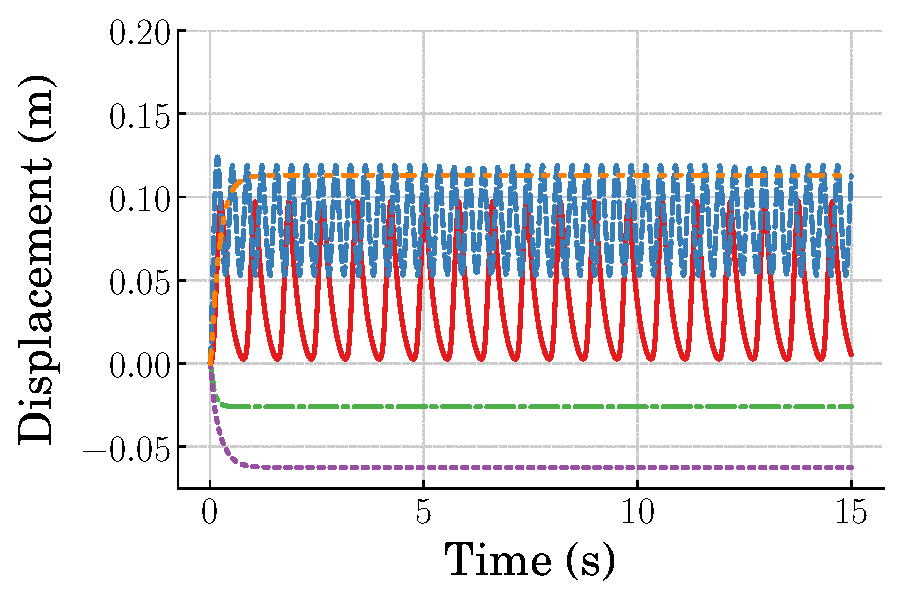
\includegraphics[width=\textwidth]{figures/figures_stability/time_responses_duffing/duffing_pure_RL/Displacement_0_init_10000_steps.pdf}
      \caption{Pure RL}
      \label{subfig_chap3:duffing_pure_RL_near_equil}
  \end{subfigure}\\
  \hfill
  \begin{subfigure}[b]{0.49\textwidth}
    \centering
    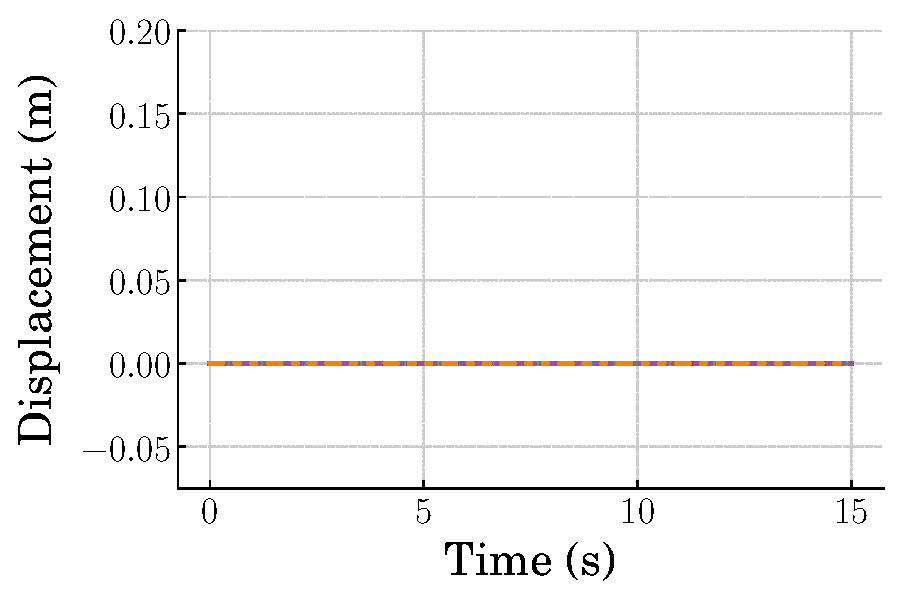
\includegraphics[width=\textwidth]{figures/figures_stability/time_responses_duffing/duffing_RL_PD/Displacement_0_init_10000_steps.pdf}
    \caption{RL-PD}
    \label{subfig_chap3:duffing_RL_PD_near_equil}
  \end{subfigure}
  \hfill
  \begin{subfigure}[b]{0.49\textwidth}
    \centering
    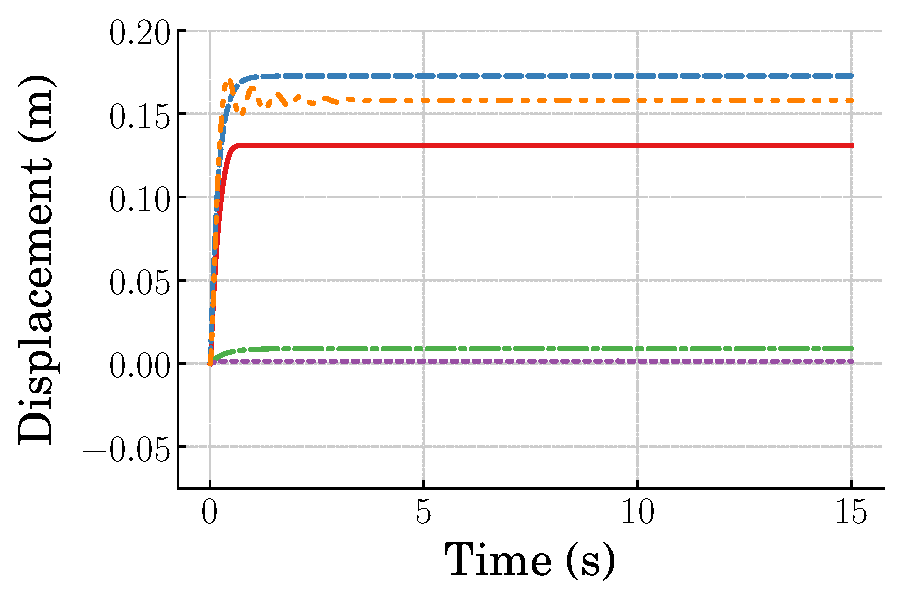
\includegraphics[width=\textwidth]{figures/figures_stability/time_responses_duffing/duffing_RL_LA/Displacement_0_init_10000_steps.pdf}
    \caption{RL-LA}
    \label{subfig_chap3:duffing_RL_LA_near_equil}
  \end{subfigure}
  \caption{Duffing oscillator response near equilibrium}
  \label{fig_chap3:duffing_near_equil}
\end{figure}
%
The Pure RL case in Figure~\ref{subfig_chap3:duffing_pure_RL_near_equil} has some responses that settle to a fixed non-zero displacement and some that have residual oscillation.
%
The responses from RL-PD in Figure~\ref{subfig_chap3:duffing_RL_PD_near_equil} have zero steady-state error and no residual oscillation
since the initial displacement and desired setpoint are equal. Figure~\ref{subfig_chap3:duffing_RL_LA_near_equil} shows the responses from RL-LA. Two of the responses have low steady-state error, while three of the responses have higher steady-state error. Although there are RL-LA responses with higher steady-state error than that of Pure RL, the RL-LA responses have no residual oscillation.
% The steady-state error from these responses are all positive, reflecting the fact that the setpoints during training are between $0$ and $1$.
%
\begin{table}[tb]
  \begin{center}
    \setlength{\tabcolsep}{6pt}
    \caption{Duffing Oscillator Stability}
    \begin{tabular}{ l c c c }
    \hline\hline
    \multicolumn{4}{c}{\textbf{Displacement Error}}\\
    \hline
    & Pure RL & RL-PD & RL-LA\\
    \hline
    \textbf{Mean} & 0.085\si{\meter} & $\textbf{0.0}$\si{\meter} & 0.097\si{\meter}\\
    \textbf{SD}  & 0.078\si{\meter} & $\textbf{0.0}$\si{\meter} & 0.077\si{\meter}\\
    \hline\hline
    \multicolumn{4}{c}{\textbf{Phase Bounds}}\\
    \hline
    & Pure RL & RL-PD & RL-LA\\
    \hline
    \textbf{Mean} & 0.554 & $\textbf{0.0}$ & 0.448\\
    \textbf{SD}  & 0.324 & $\textbf{0.0}$ & 0.365\\
    \hline
    \label{table:duffing_near_stablility}
    \end{tabular}
    % \vspace{-0.2in}
    \end{center}
  \end{table}
%
%
\begin{figure}[h!]
  \centering
  \begin{subfigure}[b]{0.49\textwidth}
      \centering
      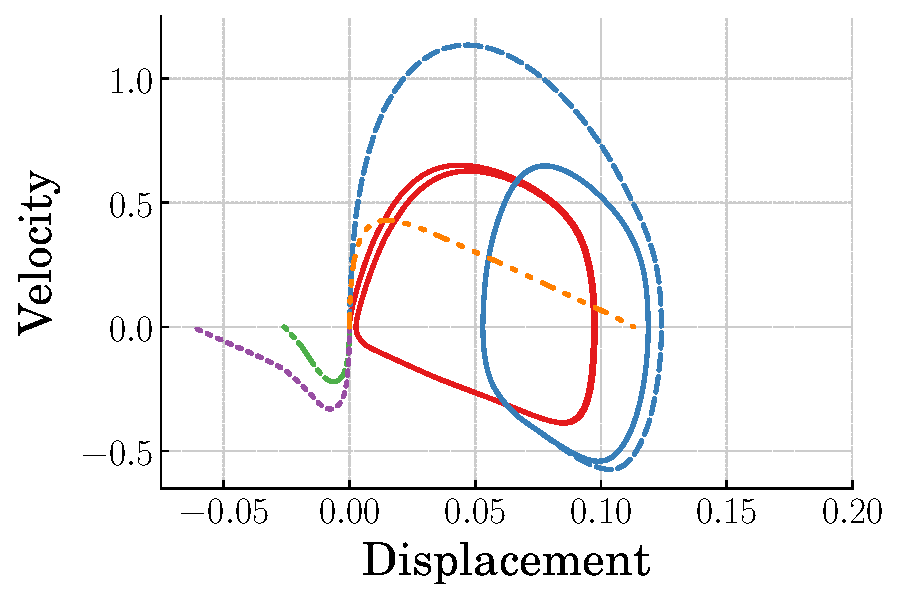
\includegraphics[width=\textwidth]{figures/figures_stability/time_responses_duffing/duffing_pure_RL/duffing_pure_RL_phase_plots.pdf}
      \caption{Pure RL}
      \label{subfig_chap3:duffing_pure_RL_phase_plot}
  \end{subfigure}\\
  \hfill
  \begin{subfigure}[b]{0.49\textwidth}
    \centering
    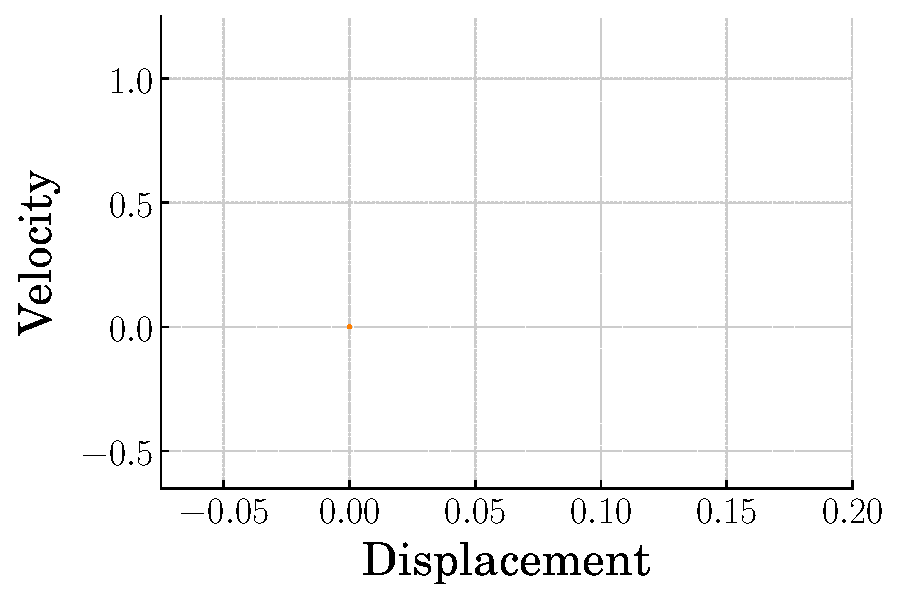
\includegraphics[width=\textwidth]{figures/figures_stability/time_responses_duffing/duffing_RL_PD/duffing_RL_PD_phase_plots.pdf}
    \caption{RL-PD}
    \label{subfig_chap3:duffing_RL_PD_phase_plot}
  \end{subfigure}
  \hfill
  \begin{subfigure}[b]{0.49\textwidth}
    \centering
    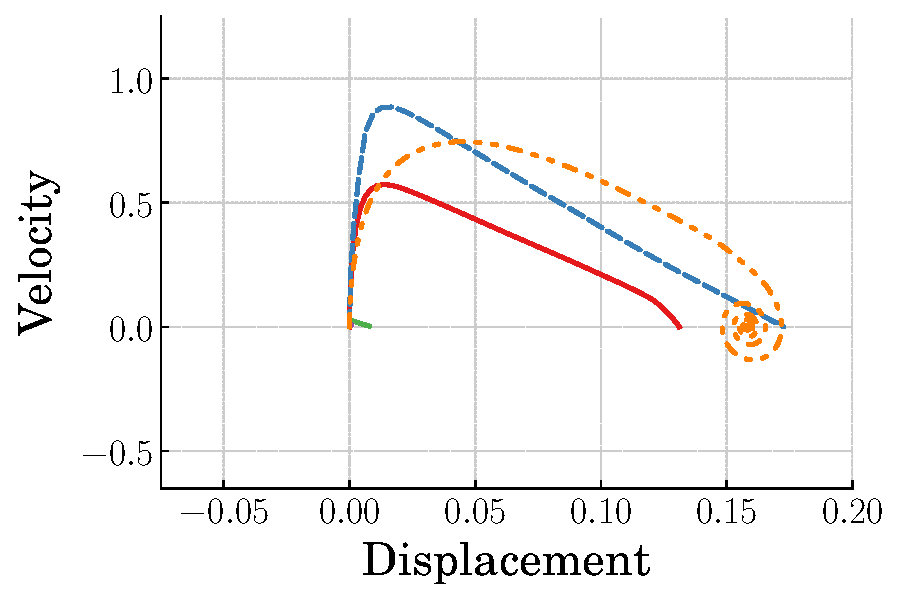
\includegraphics[width=\textwidth]{figures/figures_stability/time_responses_duffing/duffing_RL_LA/duffing_RL_LA_phase_plots.pdf}
    \caption{RL-LA}
    \label{subfig_chap3:duffing_RL_LA_phase_plot}
  \end{subfigure}
  \caption{Duffing oscillator phase responses}
  \label{fig_chap3:duffing_phase_plot}
\end{figure}
%

The minimum bounds on the displacement error for which the responses were BIBO stable were determined by the maximum displacement from each response. The mean of the absolute values and standard deviations of the bounds are summarized in Table~\ref{table:duffing_near_stablility}. RL-PD has zero steady-state error. Although the responses from Pure RL have higher residual oscillation amplitude, the mean of the maximum displacements is lower than that of RL-LA. However, the standard deviation of the maximum displacements is slightly higher for Pure RL compared to RL-LA.

Phase plots of the displacement and velocity for the duffing oscillator responses are shown in Figure~\ref{fig_chap3:duffing_phase_plot}. These were used to determine the bounds, $\epsilon$, for which the system with the different controllers was Lyapunov stable. The responses from Pure RL in Figure~\ref{subfig_chap3:duffing_pure_RL_phase_plot} show that the two responses with residual oscillation have stable limit cycles. The RL-PD responses in Figure~\ref{subfig_chap3:duffing_RL_PD_phase_plot} do not move from the initial displacement as was shown previously. Although some of the RL-LA responses in Figure~\ref{subfig_chap3:duffing_RL_LA_phase_plot} have higher maximum displacement than that of Pure RL, they have lower maximum velocities and do not exhibit limit cycles.
%
Table~\ref{table:duffing_near_stablility}
which contained the summary of BIBO stability for the controllers also
contains the mean and standard deviation of the minimum bounds for which the system satisfies Lyapunov stability.
% The stability results from the phase plots for the duffing oscillator are also summarized in Table~\ref{table:duffing_near_stablility}, where the mean of the smallest bound that satisfies Lyapunov stability and the standard deviation of those bounds are listed.
Although RL-LA has a higher mean displacement error, the mean Lyapunov bound for the Pure RL case has a larger radius due to the higher velocities of the responses.

\subsection{Double-Pendulum Crane Stability}

This section presents the stability analysis of the double-pendulum crane near the equilibrium. The controllers for the crane that were introduced in the previous chapter were:
%
\begin{align*}
  &\qquad\qquad\text{Pure RL:} & u&=a_t \qquad\qquad\qquad\\
  &\qquad\qquad\text{RL-PD:} & u&=k_px+k_d\dot{x} + \boldsymbol{a}_t\boldsymbol{\theta} \qquad\qquad\qquad\\
  &\qquad\qquad\text{RL-LA:} & u&=k_px+k_d\dot{x} + a_t \qquad\qquad\qquad\\
  &\qquad\qquad\text{RL-PD-LA:} & u&=k_px+k_d\dot{x} + \boldsymbol{a}_t\boldsymbol{\theta} + a_t \qquad\qquad\qquad
\end{align*}
%
where the acceleration command, $u$, for Pure RL is determined by the agent action, $a_t$. The other controllers utilize fixed-gain terms to bring the trolley to the desired displacement. RL-PD combines the fixed-gain terms with an agent-driven gain-scheduling controller for the pendulum states, where $\boldsymbol{a}_t$ is a vector of gains and $\boldsymbol{\theta}$ is a vector of hook and payload angular displacement and angular velocity. RL-LA uses the fixed-gain terms combined with a lumped action term and RL-PD-LA uses the fixed-gain terms in addition to both agent-driven gain scheduling and a lumped action. The stability was evaluated with the crane at rest and initial trolley and pendulum displacements of zero. The desired displacement of the trolley was also zero.
%
% (The RL-PD case has a small initial trolley displacement so that the controller output is not always zero.)
%
\begin{figure}[tb]
  \centering
  \begin{subfigure}[b]{0.49\textwidth}
      \centering
      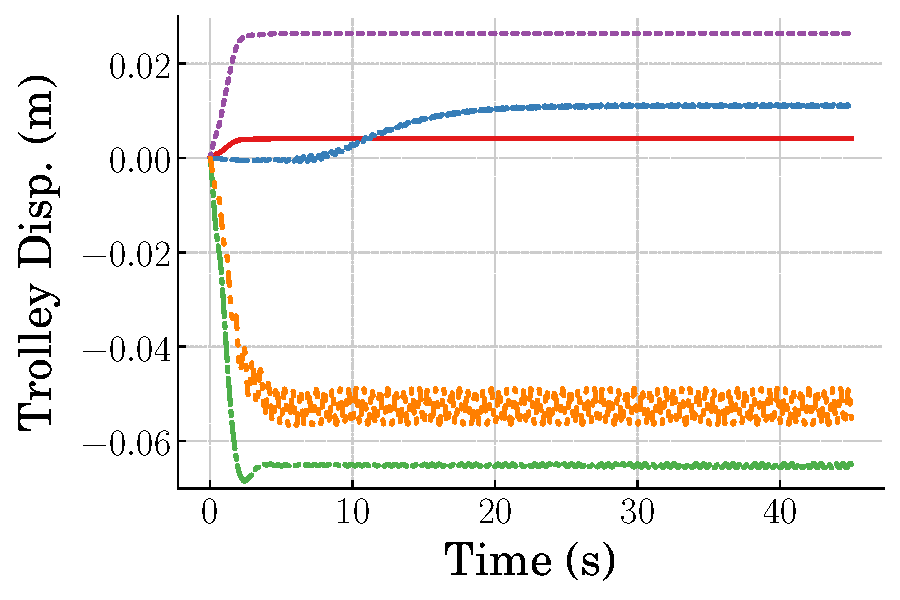
\includegraphics[width=\textwidth]{figures/figures_stability/time_responses_crane/dpcrane_pure_RL/Cart_displacement_0_init_300000_steps.pdf}
      \caption{Pure RL}
      \label{subfig_chap3:dpcrane_RL_alone_near_equil_trolley}
  \end{subfigure}
  \hfill
  \begin{subfigure}[b]{0.49\textwidth}
    \centering
    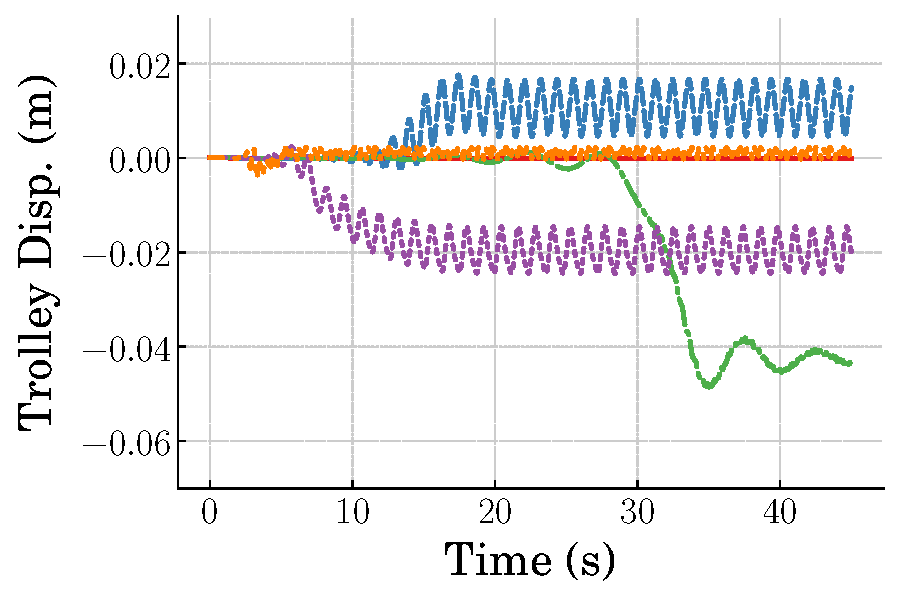
\includegraphics[width=\textwidth]{figures/figures_stability/time_responses_crane/dpcrane_cont_gain_sched/Cart_displacement_0.0001_init_300000_steps.pdf}
    \caption{RL-PD}
    \label{subfig_chap3:dpcrane_RL_PD_near_equil_trolley}
  \end{subfigure}
  \hfill
  \begin{subfigure}[b]{0.49\textwidth}
    \centering
    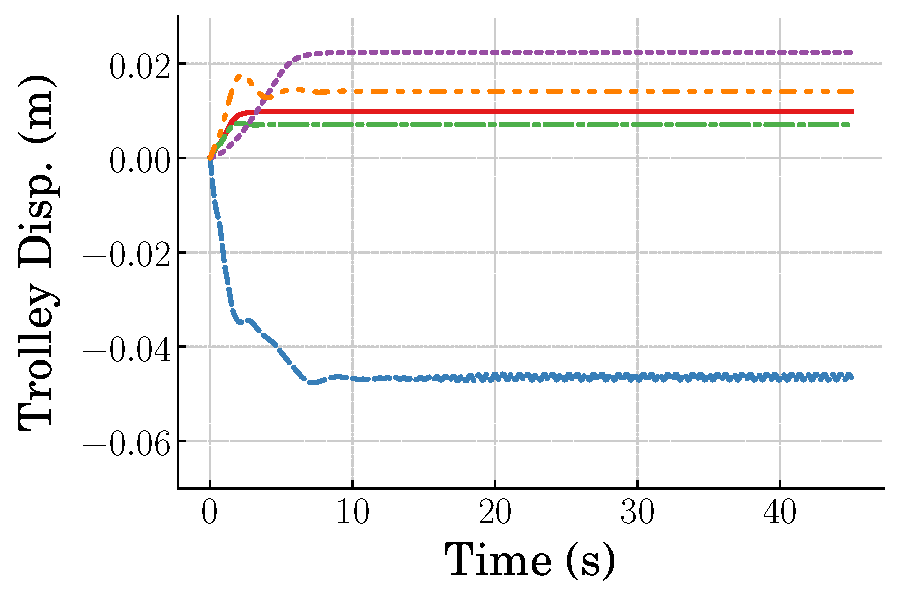
\includegraphics[width=\textwidth]{figures/figures_stability/time_responses_crane/dpcrane_RL_LA/Cart_displacement_0_init_300000_steps.pdf}
    \caption{RL-LA}
    \label{subfig_chap3:dpcrane_RL_LA_near_equil_trolley}
  \end{subfigure}
  \hfill
  \begin{subfigure}[b]{0.49\textwidth}
      \centering
      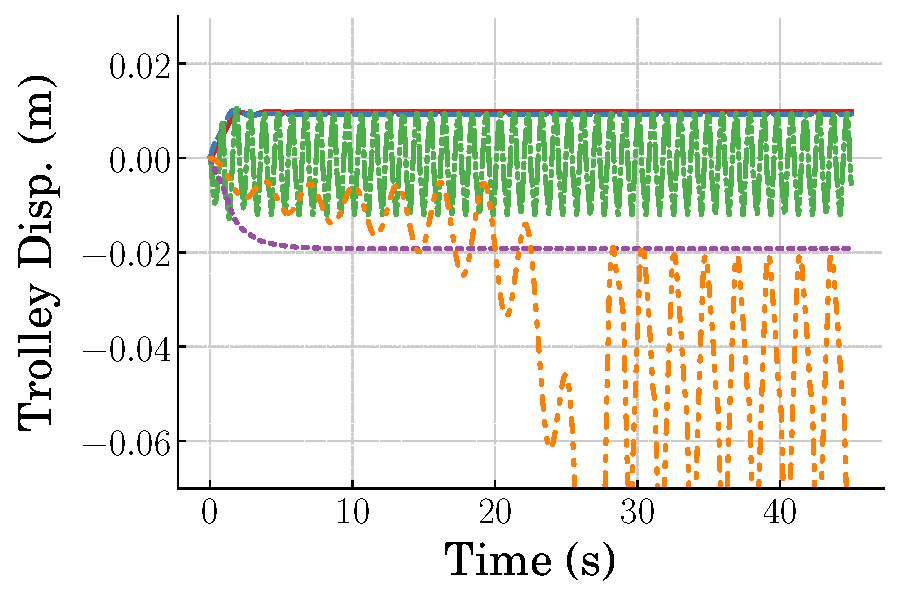
\includegraphics[width=\textwidth]{figures/figures_stability/time_responses_crane/dpcrane_RL_PD_LA/Cart_displacement_0_init_300000_steps.pdf}
      \caption{RL-PD-LA}
      \label{subfig_chap3:dpcrane_RL_PD_LA_near_equil_trolley}
  \end{subfigure}
  \hfill
  \caption{Near equilibrium trolley behavior}
  \label{fig_chap3:dpcrane_near_equil_trolley}
\end{figure}
%

The time responses of the trolley are shown in Figure~\ref{fig_chap3:dpcrane_near_equil_trolley}. The Pure RL case in Figure~\ref{subfig_chap3:dpcrane_RL_alone_near_equil_trolley} tends to have the highest steady-state error and little to no residual oscillation. For the RL-PD case in Figure~\ref{subfig_chap3:dpcrane_RL_PD_near_equil_trolley}, the error is low at the beginning of the response. However, three of the responses eventually diverge away from the equilibrium. Although RL-PD tends to have lower steady-state error, more of the responses have residual oscillation.
% Four of the five responses have steady-state error and residual oscillation.
The responses from RL-LA in Figure~\ref{subfig_chap3:dpcrane_RL_LA_near_equil_trolley} have steady-state error, but they also tend to have little to no residual oscillation compared to RL-PD.
% \rph{The responses from RL-LA in Figure~\ref{subfig_chap3:dpcrane_RL_LA_near_equil_trolley} tend to more consistently have steady-state error on the positive side of the equilibrium. Only one of the responses has residual oscillation with lower amplitude than the other cases.}
%
For the RL-PD-LA responses in Figure~\ref{subfig_chap3:dpcrane_RL_PD_LA_near_equil_trolley}, four of the five responses remain close to the equilibrium. However, the response shown in green has high residual oscillation amplitude about the equilibrium. Additionally, the response in orange slowly diverges farther from the equilibrium than the other responses until reaching a fixed steady-state error with fixed residual oscillation amplitude.
%
The minimum bounds for BIBO stability were determined by the maximum displacements of the responses. The mean and standard deviation of the bounds for the trolley are shown at the top of Table~\ref{table:dpcrane_near_stablility}.
%
\begin{table}[t]
  \begin{center}
    \setlength{\tabcolsep}{6pt}
    \caption{Planar Crane BIBO Stability}
    \begin{tabular}{ l c c c c }
    \hline\hline
    \multicolumn{5}{c}{\textbf{Trolley Displacement Error}}\\
    \hline
    & Pure RL & RL-PD & RL-LA & RL-PD-LA\\
    \hline
    \textbf{Mean} & 0.032\si{\meter} & \textbf{0.019}\si{\meter} & 0.021\si{\meter} & 0.046\si{\meter}\\
    \textbf{SD}  & 0.037\si{\meter} & \textbf{0.023}\si{\meter} & 0.025\si{\meter} & 0.072\si{\meter}\\ 
    \hline\hline
    \multicolumn{5}{c}{\textbf{Payload Displacement Error}}\\
    \hline
    & Pure RL & RL-PD & RL-LA & RL-PD-LA\\
    \hline
    \textbf{Mean} & 0.874\si{\degree} & 0.9\si{\degree} & \textbf{0.273}\si{\degree} & 1.899\si{\degree}\\
    \textbf{SD}  & 1.027\si{\degree} & 1.019\si{\degree} & \textbf{0.381}\si{\degree} & 2.662\si{\degree}\\ 
    \hline
    \label{table:dpcrane_near_stablility}
    \end{tabular}
    \vspace{-0.4in}
    \end{center}
  \end{table}
%
The maximum displacements from the RL-PD-LA controller have the highest mean and standard deviation primarily due to the response in orange in Figure~\ref{subfig_chap3:dpcrane_RL_PD_LA_near_equil_trolley}. The Pure RL case had the second-highest mean, followed by RL-LA with the second-lowest mean. RL-PD had the lowest mean bound to achieve BIBO stability.
%
\begin{figure}[t]
  \centering
  % \vspace{-1in}
  \begin{subfigure}[b]{0.49\textwidth}
      \centering
      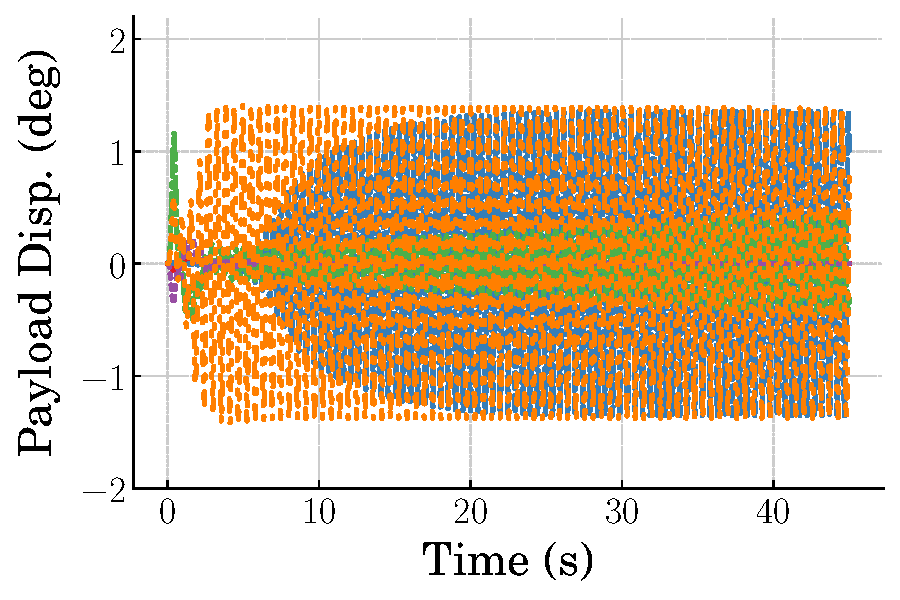
\includegraphics[width=\textwidth]{figures/figures_stability/time_responses_crane/dpcrane_pure_RL/Payload_displacement_0_init_300000_steps.pdf}
      \caption{Pure RL}
      \label{subfig_chap3:dpcrane_RL_alone_near_equil_payload}
  \end{subfigure}
  \hfill
  \begin{subfigure}[b]{0.49\textwidth}
    \centering
    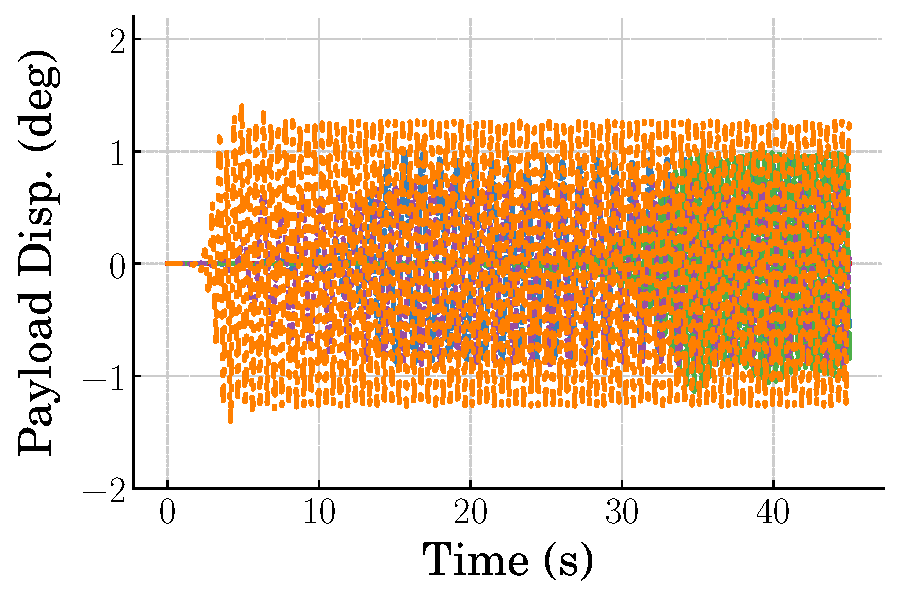
\includegraphics[width=\textwidth]{figures/figures_stability/time_responses_crane/dpcrane_cont_gain_sched/Payload_displacement_0.0001_init_300000_steps.pdf}
    \caption{RL-PD}
    \label{subfig_chap3:dpcrane_RL_PD_near_equil_payload}
  \end{subfigure}
  \hfill
  \begin{subfigure}[b]{0.49\textwidth}
    \centering
    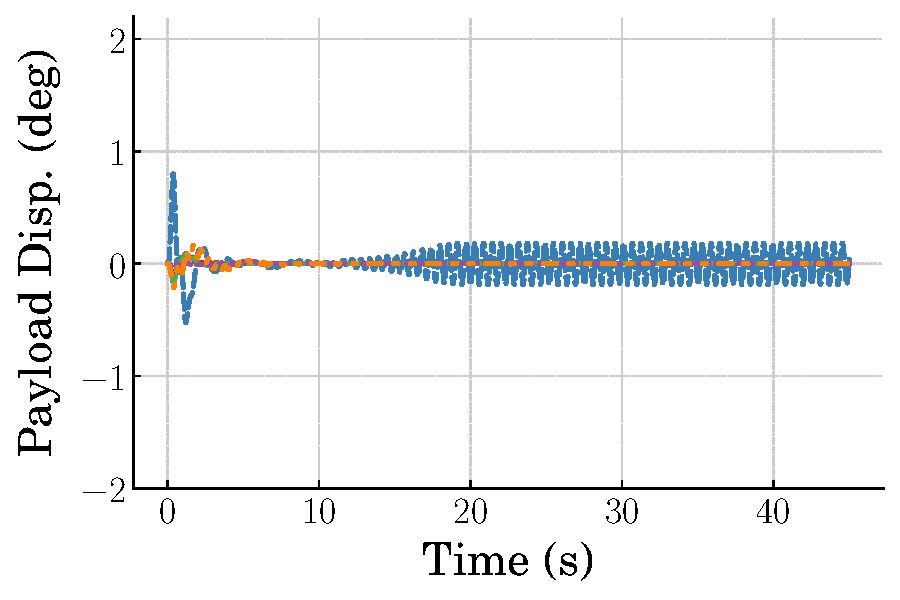
\includegraphics[width=\textwidth]{figures/figures_stability/time_responses_crane/dpcrane_RL_LA/Payload_displacement_0_init_300000_steps.pdf}
    \caption{RL-LA}
    \label{subfig_chap3:dpcrane_RL_LA_near_equil_payload}
  \end{subfigure}
  \hfill
  \begin{subfigure}[b]{0.49\textwidth}
      \centering
      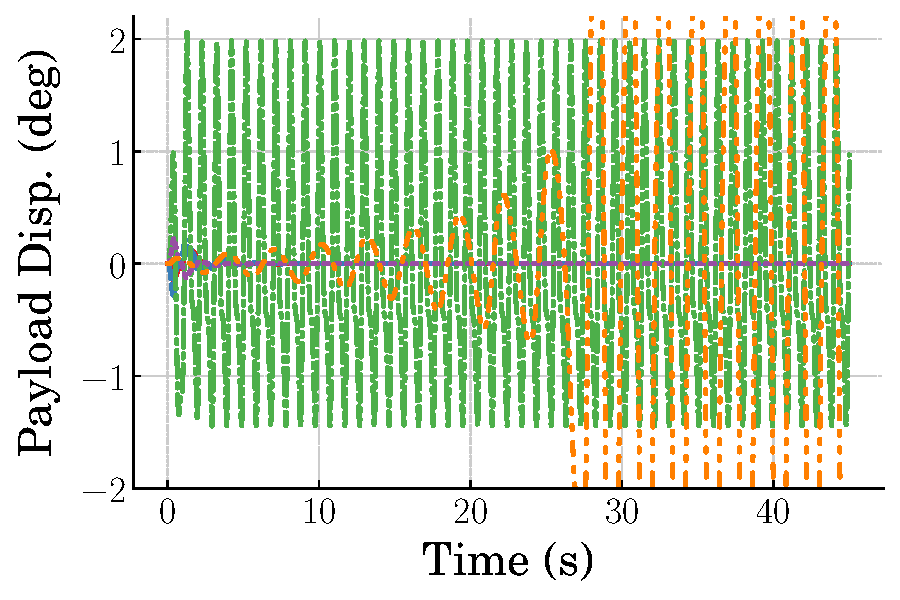
\includegraphics[width=\textwidth]{figures/figures_stability/time_responses_crane/dpcrane_RL_PD_LA/Payload_displacement_0_init_300000_steps.pdf}
      \caption{RL-PD-LA}
      \label{subfig_chap3:dpcrane_RL_PD_LA_near_equil_payload}
  \end{subfigure}
  \hfill
  \caption{Near equilibrium payload behavior}
  \vspace{-0.2in}
  \label{fig_chap3:dpcrane_near_equil_payload}
\end{figure}
%
% \FloatBarrier
%

The payload responses for the crane starting at rest with initial trolley and pendulum displacements of $x(0)=\theta(0)=0$ are shown in Figure~\ref{fig_chap3:dpcrane_near_equil_payload}. The responses from the different controllers all tended to have constant-amplitude residual oscillation.
%
Three of the five Pure RL responses in Figure~\ref{subfig_chap3:dpcrane_RL_alone_near_equil_payload} have residual oscillation, whereas four of the five RL-PD responses in Figure~\ref{subfig_chap3:dpcrane_RL_PD_near_equil_payload} have residual oscillation.
The RL-LA responses in Figure~\ref{subfig_chap3:dpcrane_RL_LA_near_equil_payload} have significantly lower residual oscillation amplitude than the other controllers.
% , where only one of the RL-LA responses has residual oscillation.
%
% The RL alone responses in Figure~\ref{subfig_chap3:dpcrane_RL_LA_near_equil_payload} and the controllers that include a continuous-gain-scheduling PD term for the pendulum states tend to have higher oscillation amplitude than the RL-LA responses in Figure~\ref{subfig_chap3:dpcrane_RL_LA_near_equil_payload}.
%
Three of the five RL-PD-LA responses in Figure~\ref{subfig_chap3:dpcrane_RL_PD_LA_near_equil_payload} have no residual oscillation, whereas two of the responses have much higher oscillation amplitude. The performance of the crane payload is summarized in the bottom half of Table~\ref{table:dpcrane_near_stablility}. The mean and standard deviation of the bounds is highest for RL-PD-LA. This is primarily caused by the two responses with high residual oscillation amplitude. The Pure RL and RL-PD controllers have similar mean and standard deviation. RL-LA has the lowest mean and standard deviation.

The trolley time responses that were previously shown are presented as phase diagrams in Figure~\ref{fig_chap3:dpcrane_near_equil_phase_trolley}. The plots show that many of the responses have limit cycles. However, there is also variance in the responses for each controller. The Pure RL responses in Figure~\ref{subfig_chap3:dpcrane_pure_RL_phase_trolley} tend to have low amplitude oscillation. However, the response in orange has a larger limit cycle with higher velocity. The RL-PD responses in Figure~\ref{subfig_chap3:dpcrane_RL_PD_phase_trolley} tend to have larger limit cycles with higher amplitude in both trolley displacement and velocity. The RL-LA responses in Figure~\ref{subfig_chap3:dpcrane_RL_LA_phase_trolley} do not have limit cycles and have less variance in displacement and velocity except for the response in blue, which travels in the opposite direction as the other responses. The RL-PD-LA phase plot responses are shown in Figure~\ref{subfig_chap3:dpcrane_RL_PD_LA_phase_trolley}. It should be noted that the plot window for this figure is larger than for the other figures. Although three of the RL-PD-LA responses have low displacement and velocity, the responses in green and orange have large and nonsmooth limit cycles.
%
\begin{figure}[tb]
  \centering
  \begin{subfigure}[b]{0.49\textwidth}
      \centering
      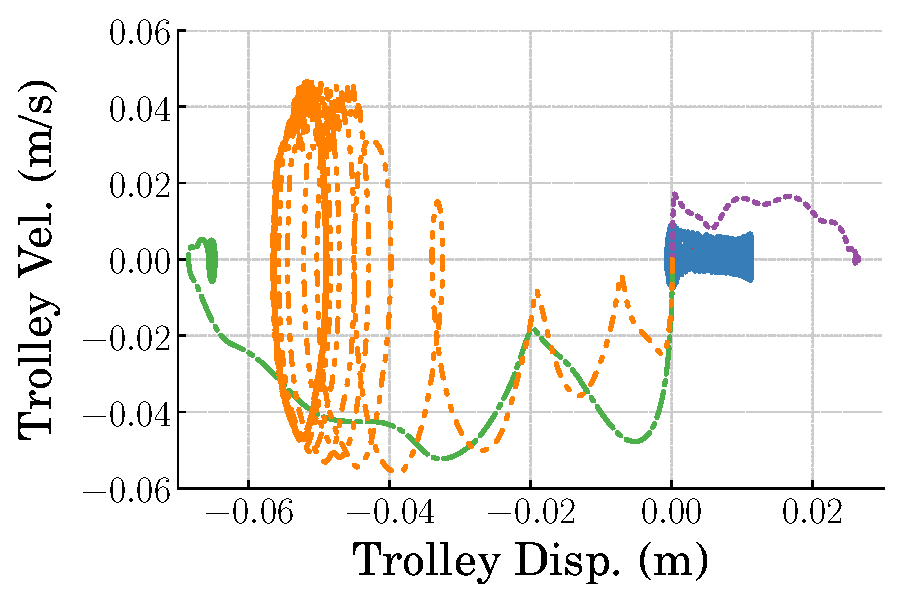
\includegraphics[width=\textwidth]{figures/figures_stability/time_responses_crane/dpcrane_pure_RL/dpcrane_pure_RL_trolley_phase_plots.pdf}
      \caption{Pure RL}
      \label{subfig_chap3:dpcrane_pure_RL_phase_trolley}
  \end{subfigure}
  \hfill
  \begin{subfigure}[b]{0.49\textwidth}
    \centering
    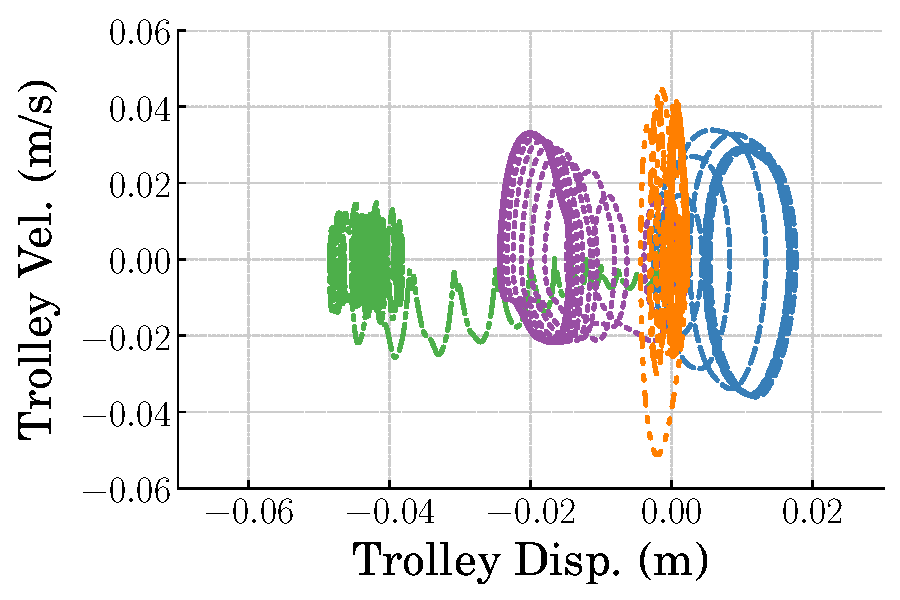
\includegraphics[width=\textwidth]{figures/figures_stability/time_responses_crane/dpcrane_cont_gain_sched/dpcrane_cont_gain_sched_trolley_phase_plots.pdf}
    \caption{RL-PD}
    \label{subfig_chap3:dpcrane_RL_PD_phase_trolley}
  \end{subfigure}
  \hfill
  \begin{subfigure}[b]{0.49\textwidth}
    \centering
    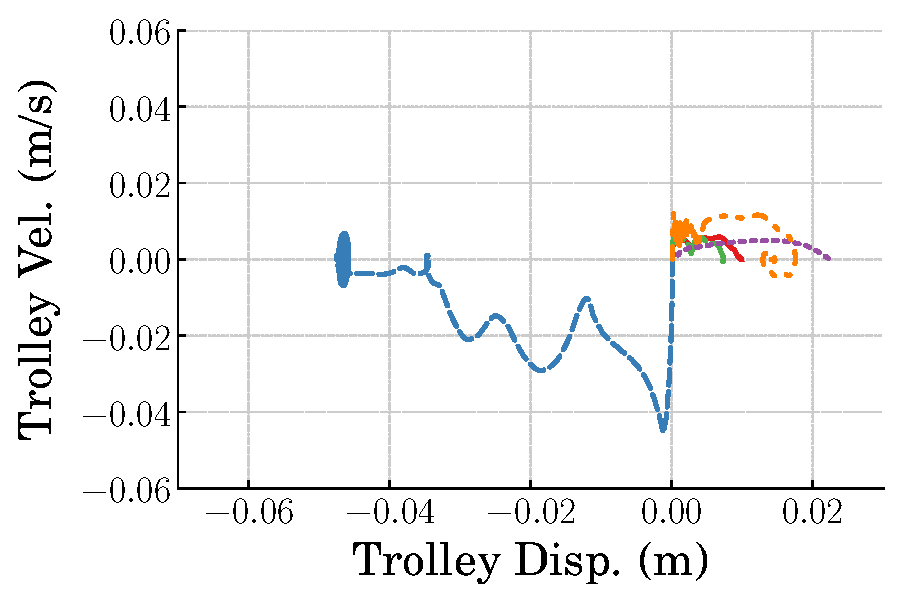
\includegraphics[width=\textwidth]{figures/figures_stability/time_responses_crane/dpcrane_RL_LA/dpcrane_RL_LA_trolley_phase_plots.pdf}
    \caption{RL-LA}
    \label{subfig_chap3:dpcrane_RL_LA_phase_trolley}
  \end{subfigure}
  \hfill
  \begin{subfigure}[b]{0.49\textwidth}
      \centering
      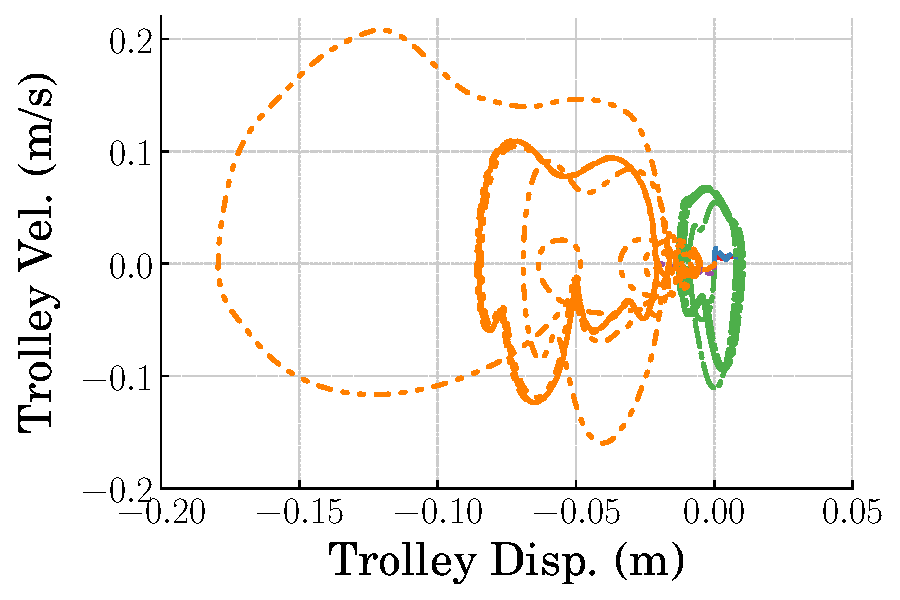
\includegraphics[width=\textwidth]{figures/figures_stability/time_responses_crane/dpcrane_RL_PD_LA/dpcrane_RL_PD_LA_trolley_phase_plots.pdf}
      \caption{RL-PD-LA}
      \label{subfig_chap3:dpcrane_RL_PD_LA_phase_trolley}
  \end{subfigure}
  \hfill
  \caption{Phase diagrams for trolley response near equilibrium}
  \label{fig_chap3:dpcrane_near_equil_phase_trolley}
\end{figure}
%
The bounds for which the trolley responses satisfy Lyapunov stability are summarized in Table~\ref{table:dpcrane_Lyapunov_stablility}. RL-LA has the smallest mean of the bounds that satisfy the stability conditions.
%
\begin{table}[h!]
  \begin{center}
    \setlength{\tabcolsep}{6pt}
    \caption{Planar Crane Lyapunov Stability}
    \begin{tabular}{ l c c c c }
    \hline\hline
    \multicolumn{5}{c}{\textbf{Trolley}}\\
    \hline
    & Pure RL & RL-PD & RL-LA & RL-PD-LA\\
    \hline
    \textbf{Mean} & 0.037 & 0.036 & \textbf{0.021} & 0.075\\
    \textbf{SD}  & 0.028 & 0.019 & \textbf{0.014} & 0.082\\ 
    \hline\hline
    \multicolumn{5}{c}{\textbf{Payload}}\\
    \hline
    & Pure RL & RL-PD & RL-LA & RL-PD-LA\\
    \hline
    \textbf{Mean} & 8.334 & 8.697 & \textbf{1.461} & 8.543\\
    \textbf{SD}  & 7.092 & 6.259 & \textbf{1.514} & 9.124\\ 
    \hline
    \label{table:dpcrane_Lyapunov_stablility}
    \end{tabular}
    \vspace{-0.2in}
    \end{center}
  \end{table}
%

%
\begin{figure}[h!]
  \centering
  \begin{subfigure}[b]{0.49\textwidth}
      \centering
      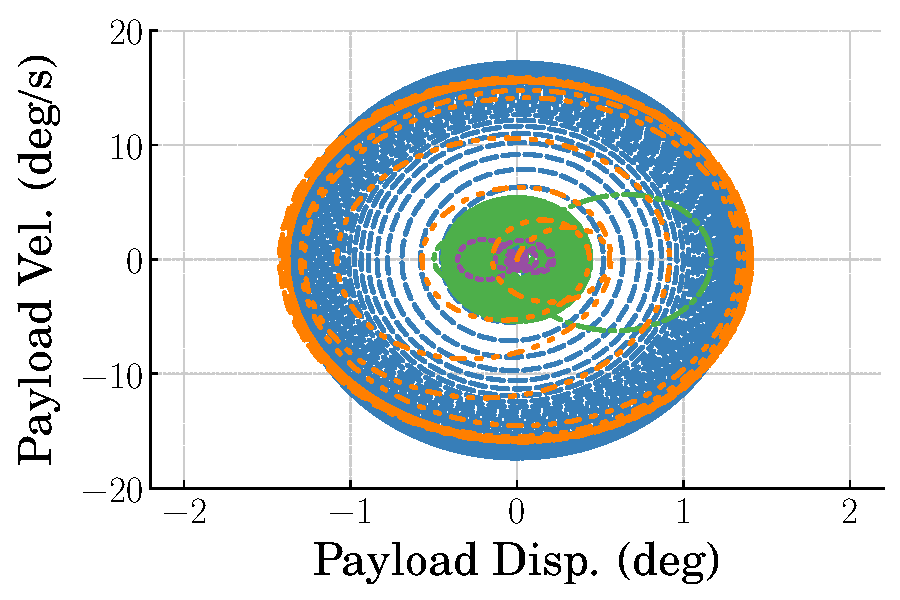
\includegraphics[width=\textwidth]{figures/figures_stability/time_responses_crane/dpcrane_pure_RL/dpcrane_pure_RL_payload_phase_plots.pdf}
      \caption{Pure RL}
      \label{subfig_chap3:dpcrane_pure_RL_phase_payload}
  \end{subfigure}
  \hfill
  \begin{subfigure}[b]{0.49\textwidth}
    \centering
    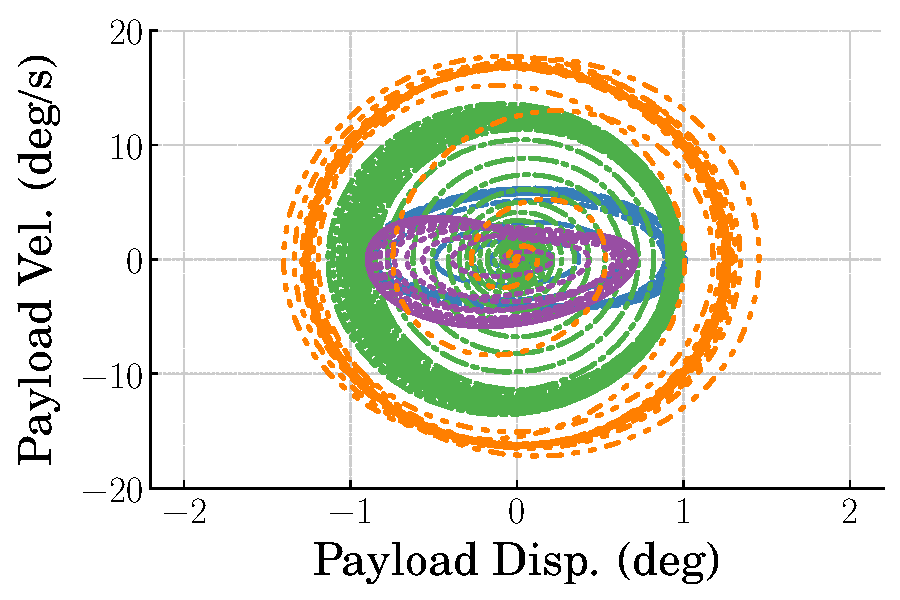
\includegraphics[width=\textwidth]{figures/figures_stability/time_responses_crane/dpcrane_cont_gain_sched/dpcrane_cont_gain_sched_payload_phase_plots.pdf}
    \caption{RL-PD}
    \label{subfig_chap3:dpcrane_RL_PD_phase_payload}
  \end{subfigure}
  \hfill
  \begin{subfigure}[b]{0.49\textwidth}
    \centering
    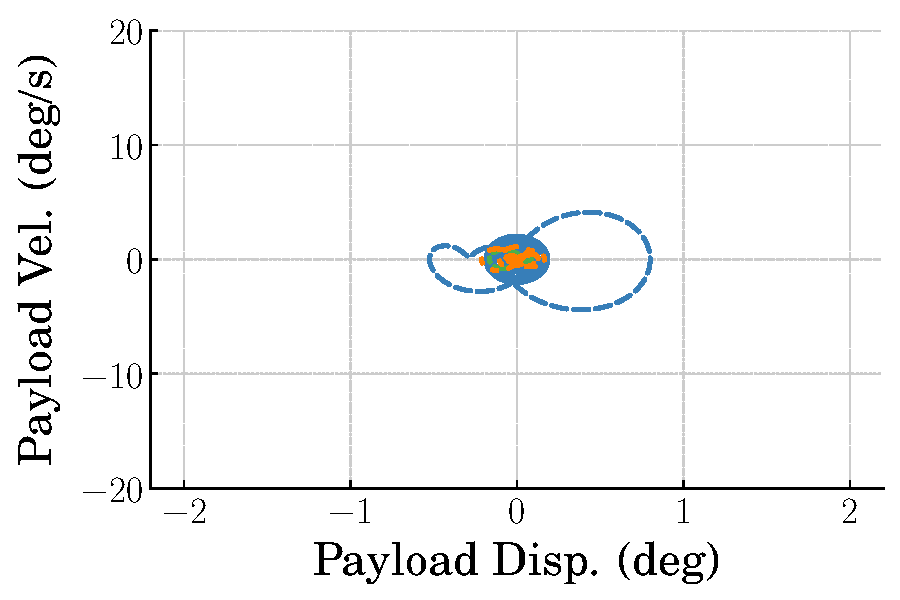
\includegraphics[width=\textwidth]{figures/figures_stability/time_responses_crane/dpcrane_RL_LA/dpcrane_RL_LA_payload_phase_plots.pdf}
    \caption{RL-LA}
    \label{subfig_chap3:dpcrane_RL_LA_phase_payload}
  \end{subfigure}
  \hfill
  \begin{subfigure}[b]{0.49\textwidth}
      \centering
      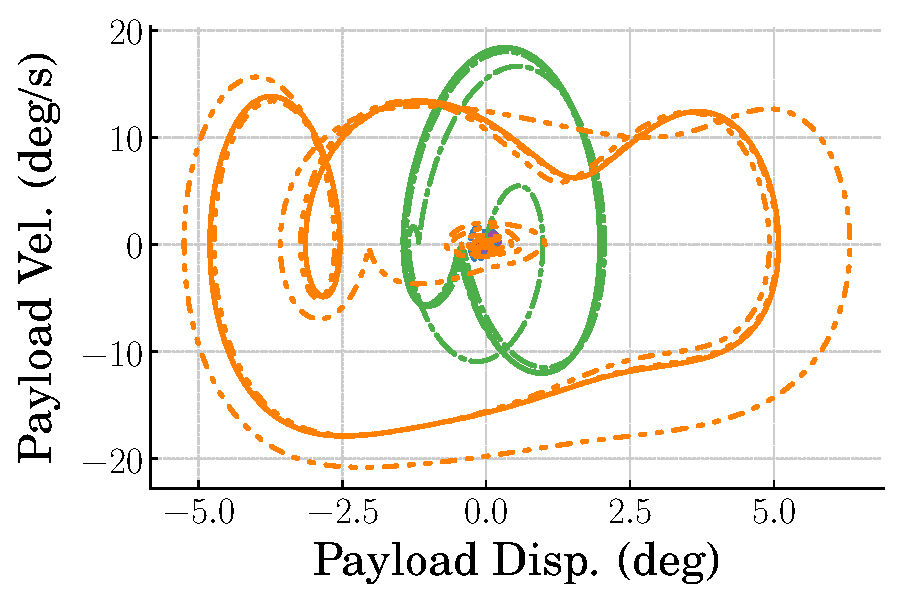
\includegraphics[width=\textwidth]{figures/figures_stability/time_responses_crane/dpcrane_RL_PD_LA/dpcrane_RL_PD_LA_payload_phase_plots.pdf}
      \caption{RL-PD-LA}
      \label{subfig_chap3:dpcrane_RL_PD_LA_phase_payload}
  \end{subfigure}
  \hfill
  \caption{Phase diagrams for payload response near equilibrium}
  \label{fig_chap3:dpcrane_near_equil_phase_payload}
\end{figure}
%
Phase diagrams for the payload responses are shown in Figure~\ref{fig_chap3:dpcrane_near_equil_phase_payload}.
The trends seen previously for the trolley responses are similar for the payload responses. The phase diagram of the RL-LA responses in Figure~\ref{subfig_chap3:dpcrane_RL_LA_phase_payload} have low displacement and velocity compared to the other controllers, corresponding to the results shown above. The payload responses for RL-PD-LA are shown in Figure~\ref{subfig_chap3:dpcrane_RL_PD_LA_phase_payload}. It should be noted that the horizontal range for the plotting window of this figure is larger than that of the other figures. Although three of the responses have low displacement and velocity, two responses have limit cycles with larger displacement amplitudes than the responses for the other cases.
%
The bounds for which the payload responses are Lyapunov stable are shown at the bottom of Table~\ref{table:dpcrane_Lyapunov_stablility}. RL-LA has the lowest mean bound and standard deviation. The other controllers have similar mean bounds for Lyapunov stability.

In summary, RL-PD had the best trolley performance in terms of BIBO stability. However, due to the tendency of the controller to excite residual oscillation, it did not perform as well for either BIBO stability of the payload or for Lyapunov stability. RL-LA consistently had the best BIBO stability of the payload and the best Lyapunov stability of the trolley and payload.


\subsection{Lyapunov Stability of Inverted Pendulum}

A stability evaluation of the inverted pendulum is presented in this section. The control laws for this system that were introduced in Chapter~\ref{chapter2} are:
%
\begin{align*}
  & \qquad\qquad\text{Pure RL:} \qquad  &u=& a_t \qquad\\
  & \qquad\qquad\text{RL-LQR:} \qquad  &u=& -k_1\theta - k_2\dot{\theta} + a_t \qquad\\
  %
  & \qquad\qquad\text{S-RL-LQR:} \qquad &u=& 
\left\{
  \begin{array}{cl}
      -k_1\theta - k_2\dot{\theta}, & \quad \forall (\theta, \dot{\theta}) \in S_{st}\\
      a_t, & \quad \forall(\theta,\dot{\theta})\notin S_{st}
  \end{array}
  \right. \qquad
\end{align*}
%
where $u$ is the acceleration input to the cart.
RL-LQR combines an action, $a_t$, from the RL agent with a fixed-gain LQR controller that is stable about the upright equilibrium at $\theta=0$. LQR and the agent operate concurrently in this controller. For S-RL-LQR, the agent controls the system for the swing up phase when the pendulum is far from the equilibrium, and LQR controls the system on its own when the pendulum is within the region of stability for LQR near the equilibrium.

Time responses for the inverted pendulum with initial conditions of $\theta(0)=\dot{\theta}(0)=0$ are shown in Figure~\ref{fig_chap3:invpend_at_equil_resp_300000steps}. Only the Pure RL and RL-LQR cases are shown since the S-RL-LQR controller does not use an RL agent term near the equilibrium. 
All of the Pure RL responses in Figure~\ref{subfig_chap3:invpend_at_equil_resp_300000steps_pure_RL} remain near the equilibrium at $\theta=0$. However, all except one of the responses have residual oscillation.
%
One of the RL-LQR responses in Figure~\ref{subfig_chap3:invpend_at_equil_resp_300000steps_RL_LQR} diverges from the equilibrium. The other responses remain near the equilibrium, but have residual oscillation.
%
\begin{figure}[tb]
  \centering
  \begin{subfigure}[b]{0.49\textwidth}
      \centering
      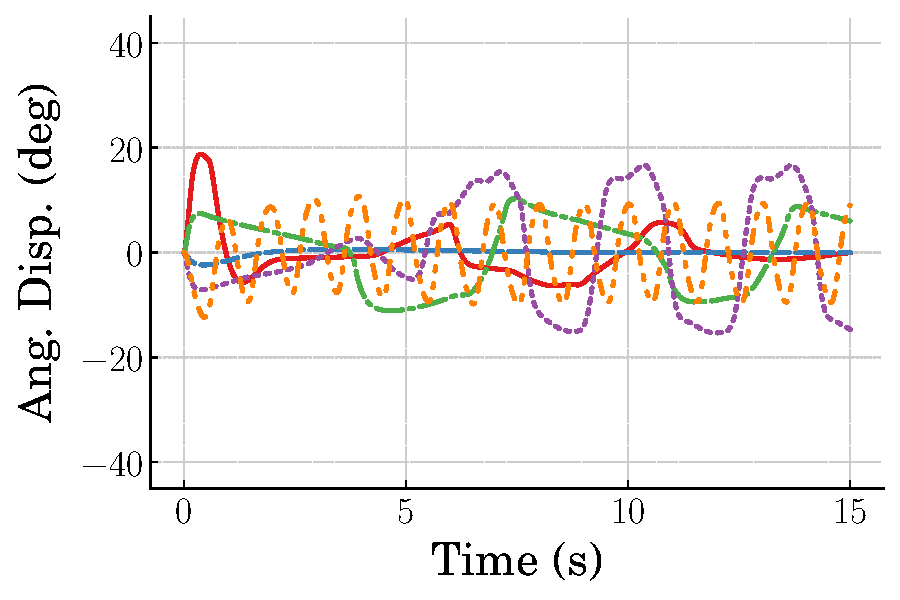
\includegraphics[width=\textwidth]{figures/figures_stability/time_responses_invpend/invpend_pure_RL/Angular_displacement_0_init_300000_steps.pdf}
      \caption{Pure RL}
      \label{subfig_chap3:invpend_at_equil_resp_300000steps_pure_RL}
  \end{subfigure}
  \hfill
  \begin{subfigure}[b]{0.49\textwidth}
      \centering
      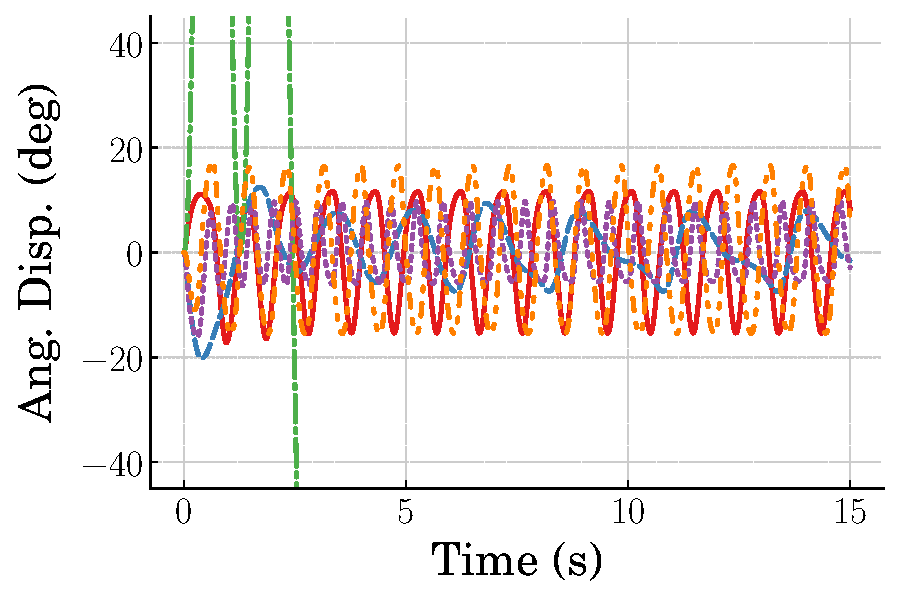
\includegraphics[width=\textwidth]{figures/figures_stability/time_responses_invpend/invpend_RL_LQR/Angular_displacement_0_init_300000_steps.pdf}
      \caption{RL-LQR}
      \label{subfig_chap3:invpend_at_equil_resp_300000steps_RL_LQR}
  \end{subfigure}
  \caption{Inverted pendulum response with initial condition at equilibrium}
  \label{fig_chap3:invpend_at_equil_resp_300000steps}
\end{figure}
%
The mean bounds for which the responses are BIBO stable are summarized in Table~\ref{table:invpend_near_stablility}. The unstable response was removed from the evaluation of RL-LQR, as indicated by the asterisk on the values. Even without the unstable response, the mean BIBO bound for RL-LQR was still higher than that of Pure RL.
\begin{table}[tb]
  \begin{center}
    \setlength{\tabcolsep}{6pt}
    \caption{Inverted Pendulum Stability, * Indicates Unstable Responses Where Removed from the Evaluation}
    \begin{tabular}{ l c c c }
    \hline\hline
    \multicolumn{4}{c}{\textbf{BIBO for Displacement}}\\
    \hline
    & Pure RL & RL-LQR & S-RL-LQR\\
    \hline
    \textbf{Mean} & 15.43\si{\degree} & $18.83\si{\degree}^*$ & \textbf{0.0}\si{\degree}\\
    \textbf{SD}  & 7.45\si{\degree} & $1.75\si{\degree}^*$ & \textbf{0.0}\si{\degree}\\
    \hline
    \multicolumn{4}{c}{\textbf{Lyapunov Bound}}\\
    \hline
    & Pure RL & RL-LQR & S-RL-LQR\\
    \hline
    \textbf{Mean} & 70.1 & $123^*$ & \textbf{0.0}\\
    \textbf{SD}  & 32.2 & $22.6^*$ & \textbf{0.0}\\
    \hline
    \label{table:invpend_near_stablility}
    \end{tabular}
    % \vspace{-0.2in}
    \end{center}
  \end{table}

Figure~\ref{fig_chap3:invpend_at_equil_phase_plot} shows the phase diagrams for the inverted pendulum responses. The responses tend to have limit cycles corresponding to the residual oscillation seen in the time responses. The maximum velocities for Pure RL in Figure~\ref{subfig_chap3:invpend_at_equil_phase_plot_pure_RL} tend to be lower than the maximum velocities for RL-LQR in Figure~\ref{subfig_chap3:invpend_at_equil_phase_plot_RL_LQR}. This corresponds to the higher frequency of the residual oscillation in the responses.
%
The bounds for which the responses are Lyapunov stable are summarized in the bottom of Table~\ref{table:invpend_near_stablility}. The unstable response was removed from the evaluation for RL-LQR, as indicated by the asterisk. The mean bound for the RL-LQR responses is higher than that of the Pure RL responses. Although the BIBO mean bound for RL-LQR is 22\% higher than that of Pure RL, the Lyapunov bound for RL-LQR was 75\% higher due to the higher velocity of the responses.
%
\begin{figure}[tb]
  \centering
  \begin{subfigure}[b]{0.49\textwidth}
      \centering
      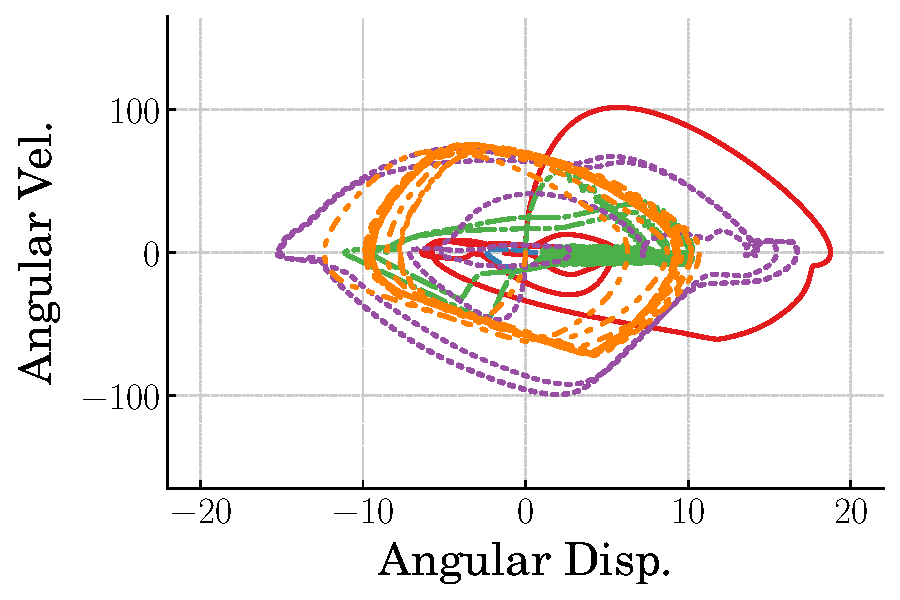
\includegraphics[width=\textwidth]{figures/figures_stability/time_responses_invpend/invpend_pure_RL/invpend_pure_RL_phase_plots.pdf}
      \caption{Pure RL}
      \label{subfig_chap3:invpend_at_equil_phase_plot_pure_RL}
  \end{subfigure}
  \hfill
  \begin{subfigure}[b]{0.49\textwidth}
      \centering
      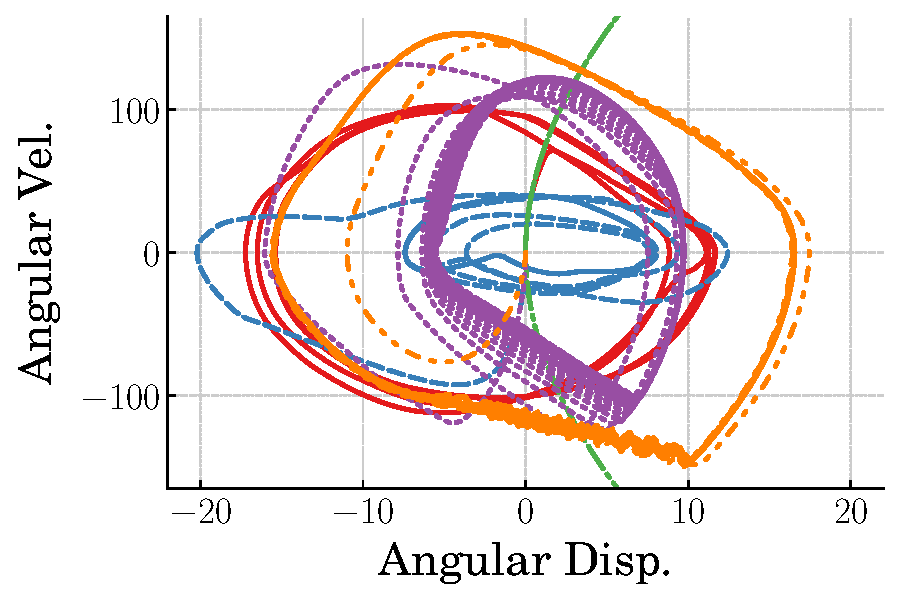
\includegraphics[width=\textwidth]{figures/figures_stability/time_responses_invpend/invpend_RL_LQR/invpend_RL_LQR_phase_plots.pdf}
      \caption{RL-LQR}
      \label{subfig_chap3:invpend_at_equil_phase_plot_RL_LQR}
  \end{subfigure}
  \caption{Inverted pendulum phase diagram from equilibrium}
  \label{fig_chap3:invpend_at_equil_phase_plot}
\end{figure}
%

S-RL-LQR had the best stability performance due to it only using LQR near the equilibrium. Pure RL had slightly better stability performance than RL-LQR when using BIBO, but it performed much better in terms of Lyapunov stability. The poor performance of RL-LQR near the equilibrium may be the result of the lack of experience of the agent near the equilibrium due to its poor performance for the swingup problem shown in Chapter~\ref{chapter2}.
% The RL-LQR agents may lack experience near the upright equilibrium due to }

%%%%%%%%%%%%%%%%%%%%%%%%%%%%%%%%%%%%%%%%%%%%%%%%%%%
% \section{Training for Stability}

% \rph{The results above show stability near equilibrium using BIBO and Lyapunov stability, which are weak notions of stability. However, the controllers were not explicitly trained for stability. Domain knowledge of the system can be utilized to train the agents to satisfy stability conditions. This section shows how knowledge of the system model and stability theory can be utilized in the design of the reward function. The results are shown for the inverted pendulum which was trained near the equilibrium to isolate the stabilization problem from the swing up problem.}

% \begin{itemize}
%   \item Previous results analyze stability near equilibrium
%   \item However, they were not trained specifically to be stable
%   \item We investigated how the design of the reward function influenced the stability properties of the agents
%   \item This was done for the inverted pendulum and trained near the equilibrium
%   \item There were quadratic reward functions used as well as Lyapunov reward function
%   \item The second method of Lyapunov is \dots
%   \item Given an energy based Lyapunov function for the inverted pendulum, the reward function is \dots
%   \item This provides a term that makes the system go towards the equilibrium and another term that rewards asymptotic stability
%   \item To provide consistency, here is the reward plot for both cases evaluated with the quadratic reward function
%   \item Here are the time responses
%   \item We get smoother responses from the Lyapunov trained case
% \end{itemize}

%%%%%%%%%%%%%%%%%%%%%%%%%%%%%%%%%%%%%%%%%%%%%%%%%%%

% \section{Asymptotic stability}

% \begin{itemize}
%   \item Lyapunov stable is a weak notion of stability
%   \item We want a stronger notion
%   \item asymptotic stability is a strong notion, but most of the agents don't achieve this
%   \item We can show this by plotting the lyapunov conditions for some time responses
%   \item We need a metric that will bridge the gap between the Lyapunov stable and asymptotically stable
% \end{itemize}

% \section{Relaxed asymptotic stability}

% \begin{itemize}
%   \item Start in some wider finite region
%   \item Go to some smaller finite region
%   \item Need to define bounds of this smaller region
%   \begin{itemize}
%     \item The bounds on the smaller region can reflect some tolerable steady-state error or oscillation
%     \item For duffing oscillator and crane, perhaps use 2\% settling time
%     \item For inverted pendulum, use stable region of LQR
%   \end{itemize}
%   \item Use system output, e.g. displacement, not full state vector
%   \item Find maximum initial output that converges to smaller bounds near equilibrium within desired time period
% \end{itemize}



% \begin{itemize}
%   \item Short comings of standard stability analysis
%   \begin{itemize}
%     \item Global stability guarantees are generally difficult/impossible for nonlinear systems
%     \item Local stability may be easier
%     \item How are the following stability criteria not useful for us
%   \end{itemize}
%   \item These include phase diagrams
%   \begin{itemize}
%     \item Phase diagrams are hard to interpret/impossible to interpret for high dimensional systems
%     \item You can find local stability, but it is impossible to figure out global stability
%     \item \what{Impossibility of guaranteeing global stability may be a general rule}
%   \end{itemize}
%   \item Stable in the sense of Lyapunov
%   \begin{itemize}
%     \item Include technical definition
%     \item Stable in the sense of Lyapunov is typically only concerned with staying within a larger set of state space given an initial condition in a smaller set of state space
%     \item I would prefer to see the controlled system move from a larger set to a smaller set near the equilibrium
%   \end{itemize}
% \end{itemize}

% \begin{itemize}
%   \item There are some methods to analyze stability of nonlinear systems
%   \begin{itemize}
%     \item Lyapunov stability
%       \begin{itemize}
%         \item Can use energy of system as Lyapunov function
%         \item The agent may be stable by some definition, but may not be asymptotically stable
%       \end{itemize}
%     \item What other methods have already been used?
%     \item I would like to be able to analyze stability even when not asymptotic
%   \end{itemize}
%   \item I can use an input/output style stability metric
%     \begin{itemize}
%       \item Many times the response converges towards a region near equilibrium
%       \item Some of the responses act a lot like a limit cycle once it gets near equilibrium
%       \item I want to measure the bounds of that limit cycle in the output variable
%       \item The problem is where do I start measuring for the bounds
%       \begin{itemize}
%         \item Instead of worrying about choosing one bound, I can use multiple bounds that show progressive damping/convergence
%         \item Place bounds at extrema
%         \item We can check how quickly the values of the extrema reduce
%         \item Allows us to mix analysis of ``asymptotic'' stability and the ``limit-cycle'' effect
%         \item I can even incorporate an estimate of the log-dec between each new extrema \rnotes{This may not work, think about this more.}
%       \end{itemize}
%     \item I will also need something to analyze how far from the desired equilibrium the actual equilibrium resides
%     \begin{itemize}
%       \item Some of the agents have a problem with bringing the system to the desired equilibrium
%       \item I can check what the agents actual equilibria are
%       \item Have to use a root finding method or similar to find it
%     \end{itemize}
%     \end{itemize}
% \end{itemize}

% % \section{Existing Stability Metrics}

% \section{BIBO}

% \what{BIBO stability is a very weak stability metric. We would much rather stronger stability guarantees like asymptotic stability, but RL agents often can't achieve that. So we are proposing an input-output stability metric that is stronger than BIBO but is not as strict as asymptotic stability.}

% \subsection{Near Equilibrium}

% \begin{itemize}
%   \item Generate time responses starting from the equilibrium
%   \item I can also plot something like a phase diagram for each coordinate and velocity
%   \begin{itemize}
%     \item This can help us figure out if it acts like a limit cycle
%     \item Plotting all five in one figure may be ok, or it may be very cramped
%   \end{itemize}
%   \item Find the bounds from each response
%   \item If I see a completely different behavior between the start at equilibrium and the start away from equilibrium, then I may be able to try the log-dec estimate
%   \begin{itemize}
%     \item Use the standard time responses from before (non-equilibrium initial condition), and plot the estimate of log-dec with time
%     \item It may be useful to generate log-dec for all coordinates
%   \end{itemize}
% \end{itemize}

% \section{Bounded-Input, Bounded-Output Inspired Stability}

% \begin{itemize}
%   \item Pick desired variable for the output
%   \begin{itemize}
%     \item This could be angular displacement for the inverted pendulum
%     \item Trolley displacement for planar crane
%   \end{itemize}
%   \item Use zero for other generalized coordinates
%   \item Near equilibrium stability
%   \begin{itemize}
%     \item Linear system will have constant decay rates, but not nonlinear systems
%     \item Agents may not always be asymptotically stable
%     \item Want to analyze decay vs time
%     \item \color{red}Learn more about nonlinear stability
%   \end{itemize}
% \end{itemize}

% \section{Asymptotic Stability}

% \begin{itemize}
%   \item Include technical definition
%   \item Requires starting somewhere (near and equilibrium) and asymptotically converging to said equilibrium
%   \item Unfortunately, most of the agents do not satisfy this requirement
%   \item They move closer to an equilibrium, but then do not asymptotically converge
%   \item Illustrate success or failure of asymptotic convergence metric for agents
%   \begin{itemize}
%     \item Use Lyapunov notion of asymptotic stability
%     \item Show that although it is stable in some sense, it does not satisfy asymptotic stability conditions
%   \end{itemize}
%   \item We're proposing a method to quantify/analyze stability for these types of systems
%   \item \what{Region of attraction is usually evaluated from an asymptotic stability perspective}
%   \item We need some way to approximate the region of attraction
% \end{itemize}

% \section{Stability of Benchmark Systems}

% \rnotes{The previous section should help us understand why it is difficult to develop generalizations about the stability (e.g. we can't achieve asymptotic stability)}

% \section{Region of Attraction}

% \what{Estimating region of attraction is always difficult.} \rnotes{We are going to look at how far away you can get and still make it into a region that we refer to as stable.}
% \begin{itemize}
%   \item Pick fixed inner bound around equilibrium
%   \item Start at initial output and see if it gets to the inner bound
%   \item Use scipy extrema to look for local max or min within bounds
% \end{itemize}

\section{Conclusion}

The stability performance of the combined controllers for the benchmark systems was evaluated using BIBO and Lyapunov stability. The performance was summarized based on the combined controller architectures introduced in Chapter~\ref{chapter2}, which were Pure RL, agent-driven gain scheduling, and fixed-gain control with RL.

The controllers with Pure RL tended to have residual oscillation and steady-state error for all of the benchmark systems. The inverted pendulum was the only system for which there was no steady-state error. There was no benchmark system for which Pure RL was the best performing controller architecture, and it instead tended to provide moderate performance.
% and the agents tended to be \rph{mid-performing}.
% \rph{Although the RL-alone controllers were never the best performing controllers for both BIBO and Lyapunov stability, they also tended not to be the worst performing.}

The stability of the agent-driven gain scheduling controllers was dependent on the benchmark system employed.
% The controllers for which the agent assigns gains at every time step \rph{had inconsistent performance that depended on the benchmark system.}
For the duffing oscillator, the RL-PD responses did not diverge from the equilibrium such that it had the best performance for both BIBO and Lyapunov stability. For the double-pendulum crane, however, the controllers with gain scheduling had good stability performance for the trolley but had moderate to poor performance for the stability bounds for the payload. This poor performance may be due to a poorly designed feedback controller rather than being a weakness of the agent-driven gain-scheduling architecture.
% \rnotes{This may be due to the gains being assigned as state feedback for the underactuated part of the system since the gains are assigned for the pendulum states.}

Combined controllers that used a fixed-gain term tended to have little to no residual oscillation; however, they often had steady-state error. For this reason, the RL-LA controller for the duffing oscillator had the largest BIBO stability bounds, but had smaller Lyapunov bounds than Pure RL. Similarly, the RL-LA stability bounds for the double-pendulum crane tended to be the smallest due to the vibration mitigation. However, RL-LQR for the inverted pendulum had the largest stability bounds, which may be related to the poor performance seen for the baseline results in Chapter~\ref{chapter2}.
% \begin{itemize}
%   \item RL alone
%   \begin{itemize}
%     \item Tended to have residual oscillation and steady-state error
%     \item Has stable limit cycles rather than damped oscillation
%   \end{itemize}
%   \item Continuous gain scheduling
%   \begin{itemize}
%     \item No error for duffing oscillator when starting at the equilibrium (asymptotically stable for non-zero initial condition)
%     \item Tends to have stable limit cycles and higher residual oscillation amplitude for double pendulum crane (Probably because the gains are on the states for the underactuated part of the system)
%   \end{itemize}
%   \item Fixed-gain and RL
%   \begin{itemize}
%     \item Tends to have little to no residual oscillation amplitude (no limit cycles)
%     \item Can still have steady-state error
%     \item Works best when fixed-gain term is stabilizing
%     \item RL-LQR (inverted pendulum) has residual oscillation, but the LQR component is not globally stabilizing
%   \end{itemize}
% \end{itemize}

Although none of the Pure RL controllers had the best stability performance, there was often a combined controller architecture that had worse performance. This suggests that combined controllers can improve stability compared to Pure RL provided that an appropriate controller architecture is used for the system.
% \rph{None of the RL-alone controllers had the best stability performance, but they often did not have the worst performance. Combined controllers can improve stability metrics compared to RL-alone controllers given the appropriate combined controller architecture for the system is used.}







